\documentclass[12pt,a4paper,frenchb]{report}

\usepackage[french]{babel}
\usepackage{a4}
\usepackage[T1]{fontenc}
\usepackage{fancyhdr}
\usepackage{multirow}
\usepackage[official]{eurosym}

%\title{FleuryMichon}
%\author{\emph{Les TouTouYouTou}}
%\date{\today}

\begin{document}

%\maketitle

\begin{minipage}{\textwidth}
\flushright{
\textbf{\Huge{\bsc{FleuryMichon}}}
\rule[+1.5ex]{\textwidth}{4pt} \\
\emph{\Large{Rapport de soutenance I}}
}
\end{minipage}
\begin{figure}[b]
\begin{center}
\large{
Sergue� \bsc{Milechine} \\
Benoit \bsc{Menet} \\
Lionel \bsc{Herbin} \\
Nicolas \bsc{Vernot} \\
}
\end{center}
\flushleft{
\emph{Les TouTouYouTou}
\rule[+1.5ex]{\textwidth}{2pt}
}
\end{figure}

\newpage

\chapter*{Introduction}

L'IRC (Internet Relay Chat) est un protocole permettant de dialoguer en temps r�el avec d'autres internautes sur un m�me serveur ou r�seau de serveurs. Pour pouvoir se connecter, les utilisateurs ont besoin d'un logiciel appel� client, � partir duquel ils peuvent, gr�ce � des commandes sp�cifiques, acc�der � des forums, plus commun�ment appel�s canaux, publiques ou priv�s. Chaque serveur d'un r�seau partage la m�me liste de canaux et d'utilisateurs. Ces r�seaux se nomment IRCnet, EFnet, DALnet \ldots Ainsi, si vous cherchez � joindre une personne en particulier, il faudra vous connecter sur le m�me r�seau. Cependant, vous n'�tes pas oblig� d'�tre sur le m�me serveur, le but �tant d'acc�der au serveur IRC le plus proche de chez vous, afin d'optimiser les temps de r�ponse.          


\newpage

\tableofcontents

\pagestyle{fancy}
\lhead{\scriptsize{\textbf{FleuryMichon} \\ \bsc{Rapport de soutenance I}}}
\rhead{\scriptsize{\bsc{Info-Sp�} \\ \bsc{Epita}}}
\headheight 18pt

\newpage

\chapter{Origine et nature du projet}

\newpage

\section{Origine du projet}

Ce soir l�, la nuit paraissait plus noire que d'habitude et les vents froids d'octobre faisaient claquer violemment les volets en bois de ma chambre. Le moment semblait id�al pour rejoindre mes amis �pit�ens, afin de partager avec eux les joies du tarot � quatre on-line. Quelques minutes de jeu ont suffit � rendre ce qui devait �tre un moment d'�panouissement personnel en r�cr�ation pour primaires en crise. En effet, la vitesse � laquelle apparaissait les insultes sur mon �cran s'approchait d'une compilation moderne. 
\\
Ainsi, nous e�mes l'id�e de cr�er notre propre ring, un monde meilleur pour le flood et autres paroles parasites. FleuryMichon �tait n�! (Ne nous demandez pas pourquoi ce nom \ldots)   

\section{Description du projet}

FleuryMichon fournira � son utilisateur un serveur (Fleury) et un client IRC (Michon). Le projet sera d�velopp� en C/C++ et utilisable sous Linux et Windows.  

\section{Composition du groupe}

\noindent Sergue� Milechine (Info-Sp� A1) \\
\verb+<milech_s@epita.fr>+ \\
\begin{footnotesize}
Projet Sup : \bsc{Bar Manager}, \emph{jeu de gestion de bar}
\end{footnotesize} \\ \\
Benoit Menet (Info-Sp� A1) \\
\verb+<menet_b@epita.fr>+ \\
\begin{footnotesize}
Projet Sup : \bsc{Mad Sheep}, \emph{jeu d'action avec des moutons}
\end{footnotesize} \\ \\
Lionel Herbin (Info-Sp� A1) \\
\verb+<herbin_l@epita.fr>+ \\
\begin{footnotesize}
Projet Sup : \bsc{BlaiRWitcH}, \emph{jeu de karting}
\end{footnotesize} \\ \\
Nicolas Vernot (Info-Sp� B1) \\
\verb+<vernot_n@epita.fr>+ \\
\begin{footnotesize}
Projet Sup : \bsc{Projet CACAGOVE}, \emph{casse-t�te/puzzle}
\end{footnotesize}


\newpage

\chapter{Etat d'avancement du serveur \emph{Fleury}}

\newpage



\section{Impl�mentation du daemon}
\section{Travaux sur les sockets}
\section{Concept de threads}
\section{Messages serveur}
\subsection{Etablissement de la connection}
\subsection{Op�rations sur les canaux}







\chapter{Etat d'avancement du client \emph{Michon}}

\newpage

\section{Programmation objet avec \emph{Qt}}
\section{Recherche bibliographique}

\newpage

\chapter{Outils de d�veloppement}

\newpage

\begin{figure}
\centering
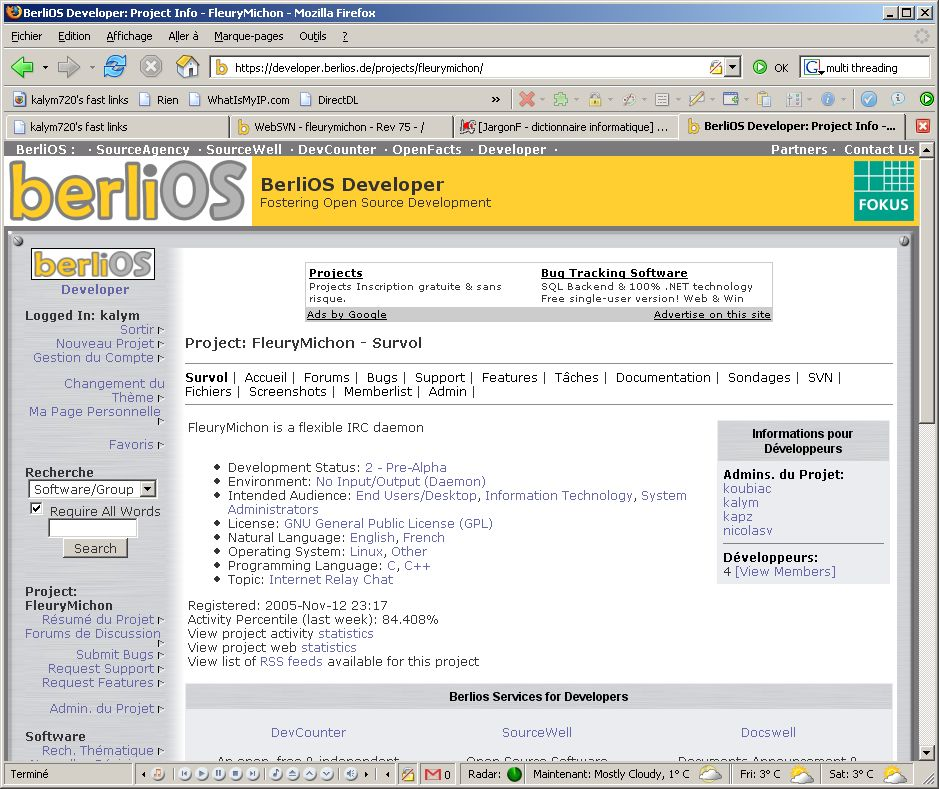
\includegraphics[width=.8\linewidth]{berlios.jpg}
\caption{Page d'accueil du projet}
\end{figure}

\begin{figure}
\centering
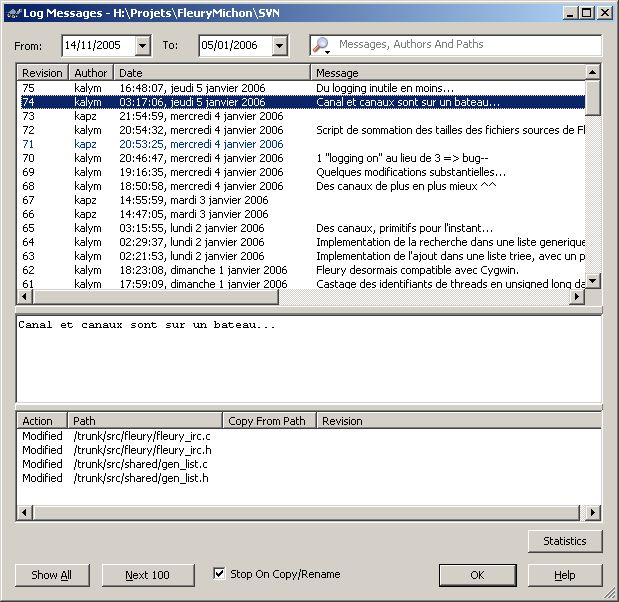
\includegraphics[width=.8\linewidth]{svn_log.jpg}
\caption{TortoiseSVN sous Windows}
\end{figure}

\begin{figure}
\centering
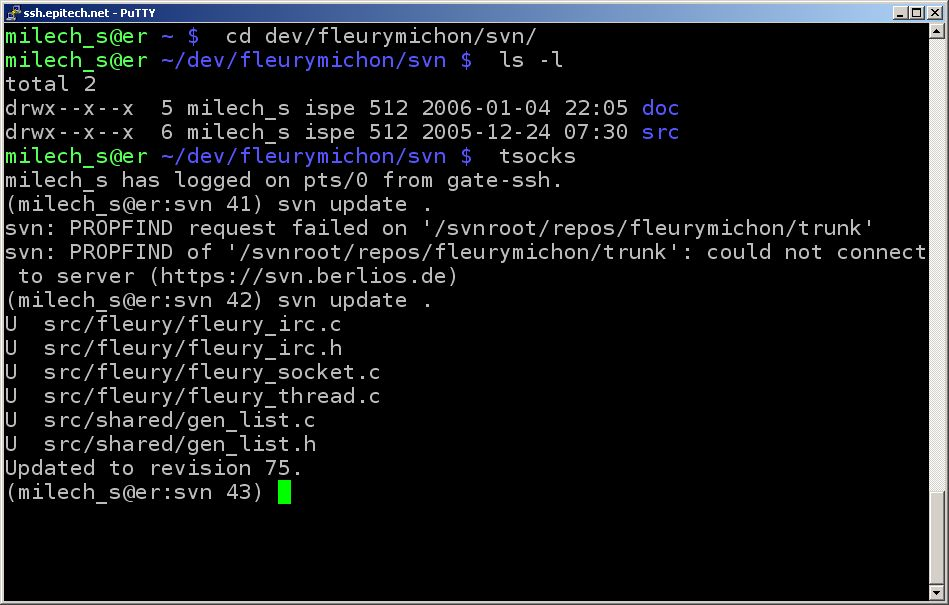
\includegraphics[width=.8\linewidth]{svn_ssh_update.jpg}
\caption{svn sous Linux, avec le proxy qui marche une fois sur deux}
\end{figure}

\section{Site Web}

Notre projet est h�berg� chez BerliOS, il s'agit d'un fournisseur de services pour d�veloppeurs qui nous apporte d'innombrables outils pour travailler sur notre projet. Nous disposons d'une interface assez compl�te permettant d'organiser l'�volution du projet, nous pouvons recevoir des demandes d'ajout de fonctionnalit�s, des demandes de support, �mettre des sondages, rapporter les bugs, discuter, publier les releases du projet, des screenshots, de la documentation \ldots 
La page d'accueil est accessible � l'adresse : (\textit{Voir Fig 4.1})\\
\verb+http://developer.berlios.de/projects/fleurymichon/+ \\

\section{Repository}

Par ailleurs, BerliOS nous offre �galement un repository Subversion. Il s'agit d'un gestionnaire de code source, qui nous permet de synchroniser notre travail � la fois rapidement et efficacement. \\
TortoiseSVN, un client graphique qui s'int�gre � l'explorateur Windows est disponible gratuitement (\textit{Voir Fig 4.2}).
Les utilitaires svn et svnadmin sont disponibles avec la majorit� des distributions Linux (\textit{Voir Fig 4.3}).


\newpage

\chapter*{Conclusion}

C�t� serveur, les TouTouYouTou n'ont pas chaum� : mise en place des sockets, gestion de la liste "client", impl�mentation des threads, gestion des canaux presque op�rationnelle.
Il nous reste donc � impl�menter les commandes manquantes ainsi que la gestion de la communication \emph{serveur-serveur}. Cependant, les travaux effectu�s sur le client n'a pas
joui d'un tel succ�s et triste est de s'aper�evoir qu'il n'y a pas encore un seul kilo-octet de source. Mais les TouTouYouTou n'ont pas dit leur dernier mot et il s'agit donc de mettre d'ores et d�j� les bouch�es double pour la prochaine
soutenance.


\end{document}
